\section{Introduction}

Since its inception, lasso regression \citep{tibshirani_1996} has quickly become a popular modeling approach due to its ability to simultaneously achieve variable selection and estimation via penalization. In the usual linear regression setting, the lasso models an $n$-dimensional vector of continuous outcomes, $\y$, as a linear combination of covariates contained in an $n$ by $p$ design matrix, $\X$, and a $p$-dimensional vector of regression coefficients, $\bb$, where the size $\bb$ is subject to an $l_1$ penalty. More precisely, the lasso estimator is defined as the minimizer, with respect to $\bb$, of the objective function:
\begin{equation*}
Q_{\text{lasso}}(\bb) = \tfrac{1}{2n}||\y - \X\bb||^2 + \lam||\bb||_1
\end{equation*}
A desirable property of the lasso estimator is that some of its components are exactly zero for sufficiently large values of the penalty parameter, $\lambda$. This allows the lasso estimate to be \textit{sparse}, with the variables corresponding to non-zero elements described as being \textit{selected} by the lasso. Unfortunately, selections made by the lasso can be unsatisfactory in certain applications, with notable examples being nominal categorical predictors or applications where basis expansions are used in non-linear additive modeling. In the former scenario, the lasso will select individual dummy variables from the design matrix rather than the underlying categorical predictors, thereby making its selections dependent upon the scheme used to encode the dummy variables and complicating efforts by the analyst to identify and interpret impactful categorical predictors. The later scenario faces a similar issue, as the overall selection status of an underlying predictor can be unclear if some columns of its basis expansion are estimated as exactly zero but others are not.

The group lasso \citep{Yuan2006} alleviates these shortcomings by imposing an $l_2$ penalty on entire groups of coefficients, resulting in selections occuring at the group level. For linear regression applications, the group lasso estimator of $\bb$ is the minimizer of:
\begin{equation*}
Q(\bb) = \tfrac{1}{2n}||\y - \X\bb||^2 + \sum_{j = 1}^{J}\lambda_j ||B_j||
\end{equation*}
This penalization framework can be extended to generalized linear models, with logistic regression \citep{meier2008} serving as a prominent example, and other likelihood-based models, such as Cox regression \citep{Wang2009}. It can also be generalized to other penalty functions, such as non-convex penalties \citep{Breheny2012}, and penalties that are also sparse at the individual coefficient level \citep{Simon2013b}. \citet{Huang2012} provides a selective review of these methods.

One potential drawback of the group lasso and related methods is the limited scope of inferential approaches that are currently available. The recently developed \textit{selective inference} \citep{Selective_Inference} family of methods has been extended to group sparse settings, including the group lasso \citep{Yang2016}, but a software implementation is only available for forward stepwise selection. Similarly, the \textit{knockoff filter} method of false discovery rate control \citep{barber2015, candes2018} has also been extended to group sparse settings \citep{Dai2016}, but it too lacks an available software implementation for group lasso models. Meanwhile, computational inferential approaches with readily available software, such as the parametric bootstrap approach implemented in the {\tt EAinference} R Package \citep{Zhou2017}, focus on the uncertainty in the individual coefficient estimates of the group lasso, rather than the selections of entire groups, limiting their utility in regards to false discovery rate control.

The focus of this paper is on the reliability of group selections made by the group lasso and its extensions. More specifically, we propose methods for controlling the marginal false discovery rate of group selections in the context of group lasso regression. We generalize our methods to variants of the group lasso, including group penalized logistic regression, other generalized linear models, and group penalized Cox regression, as well as the group MCP penalization scheme. Our proposed methods provide accessible, computationally efficient alternatives to the limited set of existing inferential approaches currently available for the group lasso. We use several simulation studies to demonstrate the robustness of these methods across a variety of data structures, as well as their ability to achieve higher true positive rates than some existing inferential approaches. 

\section{Background}

\subsection{Group lasso regression}

Consider data of the usual form, $(\y, \X)$, where $\y$ records response values for $i \in \{1, \ldots, n\}$ independent observations, and $\X$ is an $n$ by $p$ design matrix of explanatory variables. We focus on situations where the columns of $\X$ can be naturally organized into $J$ nonoverlapping groups, such that $\X = \{\X_1, \X_2, \ldots, \X_J\}$, where $\X_j$ denotes the $n$ by $K_j$ matrix containing the explanatory variables belonging to group $j$. 

The explanatory variables in $\X$ can be related with $\y$ using a probability model involving a set of coefficients, $\bb$. A well-known example is the linear regression model, which specifies the relationship:
\begin{equation}
\label{m:lin}
\y = \X\bb + \beps
\end{equation}
where $\beps$ is a $n$-dimensional vector of errors that are independent and Normally distributed with mean 0 and variance $\sigma^2$. 

Under the model described in Equation~\ref{m:lin}, the group lasso solution, $\bbh$, is the minimizer, with respect to $\bb$, of the following objective function, denoted $Q(\bb)$:
\begin{equation}
Q(\bb) = \tfrac{1}{2n}||\y - \X\bb||^2 + \sum_{j = 1}^{J}\lambda_j ||\bb_j||
\end{equation}
where $\lambda_j$ is a penalty imposed on the $l_2$-norm of the coefficients belonging group $j$. 

It is possible to specify $\lambda_j$ separately for each group, but the more common choice use $\lambda_j = \sqrt{K_j}\lambda$, which penalizes each group in accordance to its size and allows $\lambda$ to be used universally across groups. To aid in the presentation of our methods, we will assume $\lambda_j = \sqrt{K_j}\lambda$; however, this choice is not critical in any of our derivations.

The underlying framework of the group lasso can be generalized to a wide range of loss functions and penalization schemes. These variants can be expressed using the following objective function:
\begin{equation}
Q(\bb) = L(\bb|\X,\y) + \sum_{j = 1}^{J} p_{\lambda}(\bb_j)
\end{equation}
where $p_{\lambda}(\cdot)$ is a penalty function applied to each group of coefficients, and $L(\bb|\X,\y)$ is a loss function, which is based upon the log-likelihood in the case of generalized linear models, and the Cox partial likelihood in the case of Cox regression.

For sufficiently large $\lambda_j$, the elements of $\bbh_j$, the group of estimated coefficients corresponding to the columns of $\X$ that belong to group $j$ will be exactly zero. We refer to any groups whose coefficient estimates are non-zero as being ``selected" by the group lasso. Additionally, the group lasso penalty shrinks coefficient estimates towards zero, which has the benefit of allowing identifiable estimation even when the dimensionality of $\X$ is such that $p > n$.

In their original proposal, \citet{Yuan2006} assume have been orthonormalized within each group, such that $\tfrac{1}{n}\X_j^T\X_j = \I$ for all $j \in \{1, \ldots, J\}$ with $\I$ representing the identity matrix, prior to model estimation. Although data are unlikely to naturally occur in this form, groups can be orthonormalized as a pre-processing step. Provided $K_j < n$ for all $j \in \{1, \ldots, J\}$, any optimization done using the orthonormalized data is equivalent to the original scale, thus group lasso solution found on the orthonormal scale can also be easily converted back to the original scale. Throughout the remainder of this paper we assume the data have been orthonormalized within in each group as a pre-processing step. See \citet{Simon2012} for further discussion of this topic.


\subsection{Marginal false discovery rates}

Following the seminal work of \citet{BH_1995}, false discovery rate (FDR) control has become one of the most adopted inferential paradigms in applications involving large numbers of simultaneous comparisons between variables. The literature on false discovery rate control is enormous, with many authors operating under slightly different definitions. One straightforward way to define the false discovery rate is as the expected number of false selections divided by the total number of selections, which corresponds to the fraction of significant features that are expected to be false positives. Under this definition, a procedure that controls the FDR at 10\% conveys the expectation that no more than 10\% of the comparisons it identifies as significant are expected to be false positives. 

Much of the work done on false discovery rate control is in the context of \textit{large-scale univariate testing}, or applications that involve aggregating the results of a large number of single variable hypothesis tests. \citet{Farcomeni2008} and \citet{Strimmer2008} provide a more detailed overviews of these methods. Our focus is on the regression modeling framework, where the notion of a false discovery can be complicated by the presence of relationships between predictors. 

To better understand these complexities, consider the causal diagram shown below, which depicts a possible relationship between three explanatory variables, $A$, $B$, and $C$, and an outcome variable $Y$.

%\begin{figure}[!htb]
%\centering
\begin{center}
\begin{tikzpicture}[node distance=1cm]

% nodes %
\node(b)[text centered] {$B$};
\node(u)[below of = b, text centered] {$ $};
\node(a)[left of = u, text centered, xshift = -1.5cm] {$A$};
\node(c)[right of = u, text centered, xshift = 1.5cm] {$C$};
\node(y)[below of = u, text centered] {$Y$};
% edges %
\draw [arrow] (a) -- (b);
\draw [arrow] (a) -- (y);

\end{tikzpicture} \\
\end{center}
%\caption{\label{Fig:diagram} Causal diagram showing three types of relationships between variables and the outcome.}
%\end{figure}

Variable $A$ has a direct causal relationship with $Y$ and should never be considered a false discovery, while variable $C$ is independent of $Y$ and should always be considered a false discovery. Whether or not variable $B$ should be considered a false discovery less clear. In large scale univariate testing approaches, variable $B$ is not be viewed as a false discovery because it is not \textit{marginally independent} of variable $Y$, which is the criteria typically evaluated in a single variable hypothesis test. However, in the regression setting, the coefficient in the data generating model corresponding to variable $B$ would be zero, suggesting variable $B$ is a false discovery.

To clarity these distinctions, we introduce two contrasting false discovery rate perspectives: the \textit{marginal} perspective, in which a variable, or group of variables, denoted $X_j$ is a false discovery if it is declared significant despite being fully independent of the outcome: $\X_j \independent Y$, and the \textit{fully conditional} perspective, where $X_j$ is a false discovery if it is deemed significant despite being independent of the outcome conditional upon all of the other variables in the data: $X_j \independent Y | X_{k \neq j}$. Because penalized regression methods, including the group lasso, allow for only a subset of the available predictors to be active in a given model, a \textit{pathwise conditional} perspective is also possible. This perspective focuses on the model where $X_j$ first becomes active and conditions only on the other variables present in the model (a set we denote $M_j$) at that time when assessing whether or not variable $j$ is a false discovery: $X_j \independent Y | X_k \text{ for } k \in M_j$.

The methods developed in this paper use the less restrictive \textit{marginal false discovery rate} definition. While the selection of variables like $B$ in the causal diagram can be problematic in certain applications, it is often is impossible to untangle the true causal structure of the $A-B-Y$ relationship after the data have been collected. Additionally, it is always useful, regardless of application, to control the number of noise variables, like $C$, that are declared significant. For these reasons, in addition to the existing adoption of the marginal definition in the realm of large-scale univariate testing, we argue that the marginal false discovery rate is a valuable quantity to consider in applications involving the group lasso and its variants. Further, other marginal false discovery rate inferential approaches for regression models have gained traction in recent years, with \citet{Breheny2019, Miller2019, Liang2021} developing methods for the ordinary lasso, penalized GLMs and survival models, and penalized transformation models respectively.

\section{Marginal false discovery rates for the group lasso}
\label{Sec:main_meth}

\subsection{Linear regression}

Consider data generated by the usual linear model:
\begin{equation}
\y = \X\bb + \beps
\end{equation}
where $\beps$ is a $n$-dimensional vector of errors that are independent and Normally distributed with mean 0 and variance $\sigma^2$, and $\X$ is presumed to have a known grouping structure such that $\bb_j$ is a vector of length $K_j$ representing the regression coefficients associated with group $j \in \{1, \ldots, J\}$. 

Our goal is to characterize the expected number and rate falsely selected groups for a given group lasso model. We begin with the group lasso solution, $\bbh$, defined as the minimizer of the group lasso objective function, $Q(\bb)$:
\begin{equation}
Q(\bb) = \tfrac{1}{2n}||\y - \X\bb||^2 + \sum_{j = 1}^{J}\lambda_j ||B_j||
\end{equation}
Solving for $\bbh$ involves the subdifferential of $Q$ with respect to $\bb_j$:
\begin{equation}
\label{eq:kkt}
\begin{alignedat}{2}
-\tfrac{1}{n}\X_j^T(\y - \X_{-j}\bb_{-j}) + \bb_j + \lambda_j\tfrac{\bb_j}{||\bb_j||} &\quad \text{if } \bb_j &\neq 0 \\
-\tfrac{1}{n}\X_j^T(\y - \X_{-j}\bb_{-j}) + \lambda_j\mathbf{v} &\quad \text{if } \bb_j &= 0
\end{alignedat}
\end{equation}

Here, $\mathbf{v}$ is any vector satisfying $||\mathbf{v}|| < 1$, and the notation $\X_{-j}$ is used to denote the portion of $\X$ that remains after removal of the covariate group contained in $\X_j$, with $\bb_{-j}$ respectively describing the associated model coefficients. In the convex optimization literature, the criteria described in Expression~\ref{eq:kkt} are known as the KKT conditions. 

From these conditions, it follows that if the $j^{th}$ group is to be selected into the model with non-zero coefficients, it must be that the case that:
\begin{equation}
\label{eq:post_kkt}
\tfrac{1}{n}\X_j^T(\y - \X_{-j}\bbh_{-j}) - \bbh_j = \lambda_j\tfrac{\bbh_j}{||\bbh_j||}
\end{equation}

\begin{theorem}
\label{Thm:main}
For the group lasso solution $\bbh$, the component $\bbh_j \ne \zero$ if and only if

\begin{equation}
\label{eq:selc}
\tfrac{1}{n}||\X_j^T(\y - \X_{-j}\bbh_{-j})||^2 > \lambda_j^2
\end{equation}

Further, given the group $\X_j$ is marginally independent of $\y$, if $\tfrac{1}{n}\X_j^T \X_{-j}^T \inP \zero$ and $\lambda$ is chosen such that $\sqrt{n}(\bbh - \bb)$ is bounded in probability, then
\begin{equation}
\label{eq:thm1}
\tfrac{1}{n \sigma^2}||\X_j^T(\y - \X_{-j}\bbh_{-j})||^2 \inD \chi^2_{K_j}
\end{equation}
\end{theorem}

\begin{proof}
The first statement is a straightforward algebraic manipulation of Equation~\ref{eq:post_kkt}, and is a direct consequence of the KKT conditions. 

Then, expanding the left side of Expression~\ref{eq:selc} yields:
\begin{align}
\begin{alignedat}{2}
\tfrac{1}{n}||\X_j^T(\y - \X_{-j}\bbh_{-j})||^2 &= \tfrac{1}{n}||\X_j^T(\X\bb + \beps - \X_{-j}\bbh_{-j})||^2 \\
&= \tfrac{1}{n}||\X_j^T\beps - \X_j^T\X_{-j}(\bb_{-j} - \bbh_{-j})||^2 
\end{alignedat}
\end{align}
Noting $\tfrac{1}{\sqrt{n}} \X_j^T\X_{-j}(\bb_{-j} - \bbh_{-j}) \inP \mathbf{0}$ and $\beps \sim N(\zero,\sigma^2\I)$, we have $\tfrac{1}{n \sigma^2}||\X_j^T(\y - \X_{-j}\bbh_{-j})||^2 \inD \chi^2_{K_j}$.
\end{proof}

The first condition of Theorem~\ref{Thm:main}, $\tfrac{1}{n}\X_j^T \X_{-j}^T \inP \zero$, is satisfied when pairwise correlations between the columns of $\X_j$ and the other columns of $\X$ become negligible as $n$ increases. While the second condition, that $\sqrt{n}(\bbh - \bb)$ is bounded in probability, is met for suitable choices of $\lambda$ \citep{Liu2009}.

The first condition is unlikely to be met for many real data applications, instead it represents a valuable worst-case scenario regarding false discoveries. The heuristic explanation is that in penalized regression applications where two groups are related to each other, the selection of one group reduces the chances that the other is also selected. Thus, treating groups as independent will yield a conservative estimate of the marginal false discovery rate. Quantifying the exact degree of conservatism introduced by these relationships is significantly less mathematically tractable, but we extensively explore the issue via simulation study in Section~\ref{Sec:sim}. \citet{Breheny2019} presents a more detailed theoretical discussion of this topic in the context of the ordinary lasso.

\begin{clry}
\label{Clry:main}
Under the conditions outlined in Theorem~\ref{Thm:main}, for the group lasso model characterized by $\lambda$, the expected number of false discoveries and the expected rate of marginal false discoveries are respectively bounded by:
\begin{align}
\label{eq:Mfdr}
\begin{alignedat}{2}
\FD &= \sum_{j = 1}^{J} \Pr \big(\chi^2_{K_j} > \frac{n\lam_j^2}{\sigma^2}\big)\\
\mFDR &= \frac{\FD}{\text{S}} 
\end{alignedat}
\end{align}
where $\text{S}$ denotes the total number of selected groups in the model characterized by $\lambda$.
\end{clry}

Theorem~\ref{Thm:main} implies the probability that the $j^{th}$ group is selected, given the group is marginally independent of the outcome, corresponds to the probability that a $\chi^2_{K_j}$ random variable is larger than $\frac{n\lam_j^2}{\sigma^2}$. In principle, we'd then sum over all groups that are marginally independent of the outcome to determine the expected number of falsely selected groups; however, the identity of such groups is unknown in practice, so summing overall $J$ groups provides a conservative alternative. In many applications of the group lasso, the number of groups that are truly related to the outcome is small relative to the total number of groups, making this effect relatively small.

For a given value of $\lambda$, the process of calculating $\mFDR$ is summarized in Algorithm~\ref{Alg:mfdr}.

\begin{algorithm*}
\caption{Calculating the mFDR upper bound}\label{Alg:mfdr}
\begin{algorithmic}[10]
\Procedure{}{}
\State Estimate $\sigma^2$ as $\hat{\sigma}^2$
\For {\texttt{$j \in \{1, \ldots, J\}$}}
\State $\widehat{\FD}_{j, \lam} = \Pr \big(\chi^2_{K_j} > \frac{n\lam_j^2}{\hat{\sigma}^2}\big)$ by the result of Theorem 1
\EndFor
\State $\widehat{\FD}_\lam = \sum_{j=1}^{J} \widehat{\FD}_{j, \lam} $
\State $\widehat{\mFDR}_\lam = \text{min}\left(\frac{\widehat{\FD}_\lam}{S_\lam}, 1 \right)$
\EndProcedure
\State \textbf{return} $\widehat{\mFDR}_\lam $
\end{algorithmic}
\end{algorithm*}

We point out that the initial step of Algorithm~\ref{Alg:mfdr} requires estimating $\sigma^2$, either by dividing the residual sum of squares by its degrees of freedom or via the cross-validated error of the model under consideration. 

\subsection{Generalized linear models}
\label{Sec:glm}

The group lasso penalty can be extended to other likelihood-based models, such as GLMs and Cox regression. Solving for $\bbh$ in these applications typically relies upon a quadratic approximation of the log-likelihood function, $L$:
\begin{equation}
\label{eq:quad}
L(\be) = L(\bet) + (\be - \bet)^T\vv + \tfrac{1}{2}(\be - \bet)^T\W(\be - \bet)
\end{equation}
where $\eta = \X\bb$, with $\bet$ denoting the current estimate, and $\vv$ and $\W$ respectively denote the first and second derivatives of $L(\be)$ evaluated at $\bet$. It is worthwhile noting that $\W$ is a diagonal matrix in popular GLMs such as logistic regression.

Letting $\z = \bet - \W^{-1}\vv$, and dropping terms that are constant with respect to $\bb$, the approximation in Equation~\ref{eq:quad} results in a loss function that is equivalent to weighted squared error loss:
\begin{equation}
L(\bb) \approx \tfrac{1}{2}(\z - \X\bb)^T\W(\z - \X\bb)
\end{equation}
Thus, the optimization algorithms that solve for the group lasso solution, as well as the corresponding KKT conditions, can be adapted to likelihood-based models by the minor addition of a weight matrix, $\W$. 

Consequently, groups selections made by these models are characterized by the following condition:
\begin{equation}
\label{eq:sel_glm}
\tfrac{1}{n}||\X_j^T\W(\z - \X_{-j}\bbh_{-j})||^2 > \lambda_j^2
\end{equation}
Applying the same general steps previously described in the linear regression setting, we can work towards characterizing the marginal false discovery rate of these models using the left-hand side of Expression~\ref{sel_glm}:
\begin{equation}
\label{eq:Mfdr_proof_glm}
\tfrac{1}{n}||\X_j^T\W(\z - \X_{-j}\bbh_{-j})||^2 = \tfrac{1}{n}||\X_j^T\vv - \X_j^T\W\X_{-j}(\bb_{-j} - \bbh_{-j})||^2 
\end{equation}

\begin{prop}
\label{prop1}
Provided $(\X^T\W\X)^{-1/2}\X^T\vv \inD N(\zero, \I)$, where $\I$ is the $p$ x $p$ identity matrix, if $\tfrac{1}{n}\X_j^T \W \X_{-j}^T \inP \zero$, and $\sqrt{n}(\bbh- \bb)$ is bounded in probability, then the number and rate of marginal false discoveries of a likelihood-based model subjective to the group lasso penalty characterized by $\lambda$ can be estimated by:
\begin{align}
\label{eq:Mfdr_glm}
\begin{alignedat}{2}
\FD &= \sum_{j = 1}^{J} \Pr \bigg(\chi^2_{K_j} > \frac{n^2\lam_j^2}{\Tr(\X_j^T\W\X_j)}\bigg)\\
\mFDR &= \frac{\FD}{\text{S}} 
\end{alignedat}
\end{align}
\end{prop}

The first condition involved in Proposition~\ref{prop1} is a standard result of classical likelihood theory, which can be shown for many types of generalized linear models and Cox regression. The remaining conditions are direct analogs of those described in Theorem~\ref{Thm:main} for the linear regression setting. As a result, the derivations of the estimates in Equations~\ref{eq:Mfdr_glm} are analogous to those of Theorem~\ref{Thm:main} and Corollary~\ref{Clry:main}, with the primary distinction being the variance used in normalization. 

Like the linear regression setting, we can summarize the calculation of $\mFDR$ for given value of $\lambda$ in a group lasso penalized likelihood-based model using the following algorithm:

\begin{algorithm*}
\caption{Calculating the mFDR upper bound (GLMs}\label{Alg:mfdr_glm}
\begin{algorithmic}[10]
\Procedure{}{}
\State Estimate $\W \gets \nabla^2f(\beh)$
\For {\texttt{$j \in \{1, \ldots, J\}$}}
\State $\widehat{\FD}_{j, \lam} = \Pr \bigg(\chi^2_{K_j} > \frac{n^2\lam_j^2}{\Tr(\X_j^T\W\X_j)}\bigg)$ by Proposition 1
\EndFor
\State $\widehat{\FD}_\lam = \sum_{j=1}^{J} \widehat{\FD}_{j, \lam} $
\State $\widehat{\mFDR}_\lam = \text{min}\left(\frac{\widehat{\FD}_\lam}{S_\lam}, 1 \right)$
\EndProcedure
\State \textbf{return} $\widehat{\mFDR}_\lam $
\end{algorithmic}
\end{algorithm*}

As was the case in the linear regression setting, these estimates will be conservative in the presence of pairwise correlations across columns of $\X$ corresponding to different groups, and in applications were $J$ is substantially exceeds the number of groups that are marginally independent of the outcome. 

Additionally, the estimates produced by Algorithm~\ref{Alg:mfdr_glm} are subject to further uncertainty arising from the use of the average diagonal element of $\X_j^T\W\X_j$ in normalization. Section~\ref{Sec:sim} explores the reliability of these estimates via simulation study for group penalized logistic and Cox regression models under several different design matrices and correlation structures.

\subsection{Other penalty functions}

The general form of the $\mFDR$ estimators described in prior sections are directly applicable to several other penalization schemes related to the group lasso. One example is the group minimax concave penalty, or group MCP. In non-grouped applications, the MCP penalty function, $f_{\lambda, a}(\theta)$, is defined as:
\begin{equation}
\label{eq:mcp}
\begin{alignedat}{2}
\lambda\theta - \tfrac{\theta^2}{2a} &\quad \text{if } \theta &\leq a\lambda \\
\tfrac{1}{2}a\lambda^2 &\quad \text{if } \theta &> a\lambda
\end{alignedat}
\end{equation}
for values of $\lambda \geq 0$. Here, $a$ is a tuning parameter, with $a = 3$ being the typical value used in most software implementations. MCP is a concave penalty where the degree of penalization is diminished, eventually becoming zero, for large coefficients. 

In grouped applications, the composite group MCP estimate \citep{Breheny2012, Huang2012} is defined as the minimizer of:
\begin{equation}
Q(\bb) = \tfrac{1}{2n}||\y - \X\bb||^2 + \sum_{j = 1}^{J}f_{\lambda, b}\bigg(\sum_{k=1}^{K_j} f_{\lambda,a}(|\beta_{jk}|)\bigg)
\end{equation}
where the tuning parameter $b$ is typically chosen to be $K_ja\lambda/2$ to ensure that the group level penalty attains its maximum if and only if each of its components are at their maximum.

Although the coefficient estimates arising from group MCP regression tend to differ from those of the group lasso, the optimization conditions that define the entry criteria for a group becoming active in the model are identical. Consequently, the same estimators proposed in \ref{eq:Mfdr_glm1} and \ref{eq:Mfdr} can also be used to control the marginal false discovery rate in group MCP regression. In Section~\ref{Sec:sim} we present results for both the group lasso and group MCP penalties in several of the simulation experiments used to explore various aspects our proposed $\mFDR$ estimators.

\section{Simulation experiments}
\label{Sec:sim}

\subsection{Data generation}

In the following sections we present results from a variety of simulation experiments exploring the validity and efficacy of our proposed $\mFDR$ methods.  In all of these experiments, the covariates recorded in $\X$, are derived from numeric values randomly generated from a multivariate normal distribution with a mean of $\zero$ and a covariance matrix, $\Sigma_X$. The off-diagonal entries of $\Sigma_X$ are used to invoke specific correlation structures, we focus on two particular cases: Independence - $cor(\x_a \x_b) = 0$, and Autoregressive - $cor(\x_a, \x_b) = \rho^{|a - b|}$, for all $a, b \in \{i,\ldots,J\}$. After these numeric values are generated, they are then used to construct design matrices for the two primary applications we are focused on, models containing nominal categorical predictors and non-parametric additive models. 

In applications focused on categorical predictors, the final design matrix is constructed by binning the underlying numeric values into $k$ equally sized groups, which are then expressed in the design matrix using $k$ dummy variables. Outcomes are then generated from the linear model $\y = \X \bb+ \beps$, where $\epsilon_i$ is independently drawn from a $N(0,1)$ distribution, in linear regression applications, from a Bernoulli distribution with $\Pr(y_i = 1) = 1/(1 + exp(-\x_i^T\bb))$ in logistic regression applications, or from an exponential distribution with a rate parameter equal to $exp(-\x_i^T\bb)$ in Cox regression applications.

In applications focused on non-parametric additive models, outcomes are generated directly from the underlying numeric values.  For linear regression scenarios, this is done such that $\y = \sum_{j = 1}^{t} f(\x_j) + \beps$, where the function, $f$, defines a non-linear relationship between active features and the outcome, $t$ is a pre-specified number of non-noise features, and $\epsilon_i$ is independently drawn from a $N(0,1)$ distribution. For logistic regression scenarios, the outcome is drawn from a Bernoulli distribution with $\Pr(y_i = 1) = 1/(1 + exp(- \sum_{j = 1}^{t} f(\x_{ij})))$, and for Cox regression scenarios the outcome is drawn from an exponential distribution with a rate parameter equal to $exp(\sum_{j = 1}^{t} f(\x_{ij}))$. We consider two different forms of $f$: Quadratic - $f(X) = \beta X^2$, Piecewise Linear - $f(X) = \beta X$ if $X > 0$ and $f(X) = 0$ otherwise. Prior to model fitting, each feature undergoes a basis expansion with $K_j$ degrees of freedom, thereby yielding a design matrix containing $J$ groups of size $K_j$.

\subsection{False discovery rate control}

Standard software packages will fit a series group lasso models along a decreasing sequence of $\lambda$ values.  The estimators described in Equations~\ref{eq:Mfdr} and \ref{eq:Mfdr_glm} can be used to estimate the number of false discoveries that are expected in each model of this sequence. The curves displayed in Figure~\ref{Fig:lseq1} display the mean estimated number of marginal false group selections and the mean empirical number of false group selections averaged over 200 simulation repetitions along a fixed, decreasing sequence of $\lambda$ values in the piecewise linear data generation scenario for group lasso penalized linear, logistic, and Cox regression with $n = 1000$, $J = 100$, and $t = 10$ under the independence correlation structure. 

\begin{figure} [!htb]
\centering
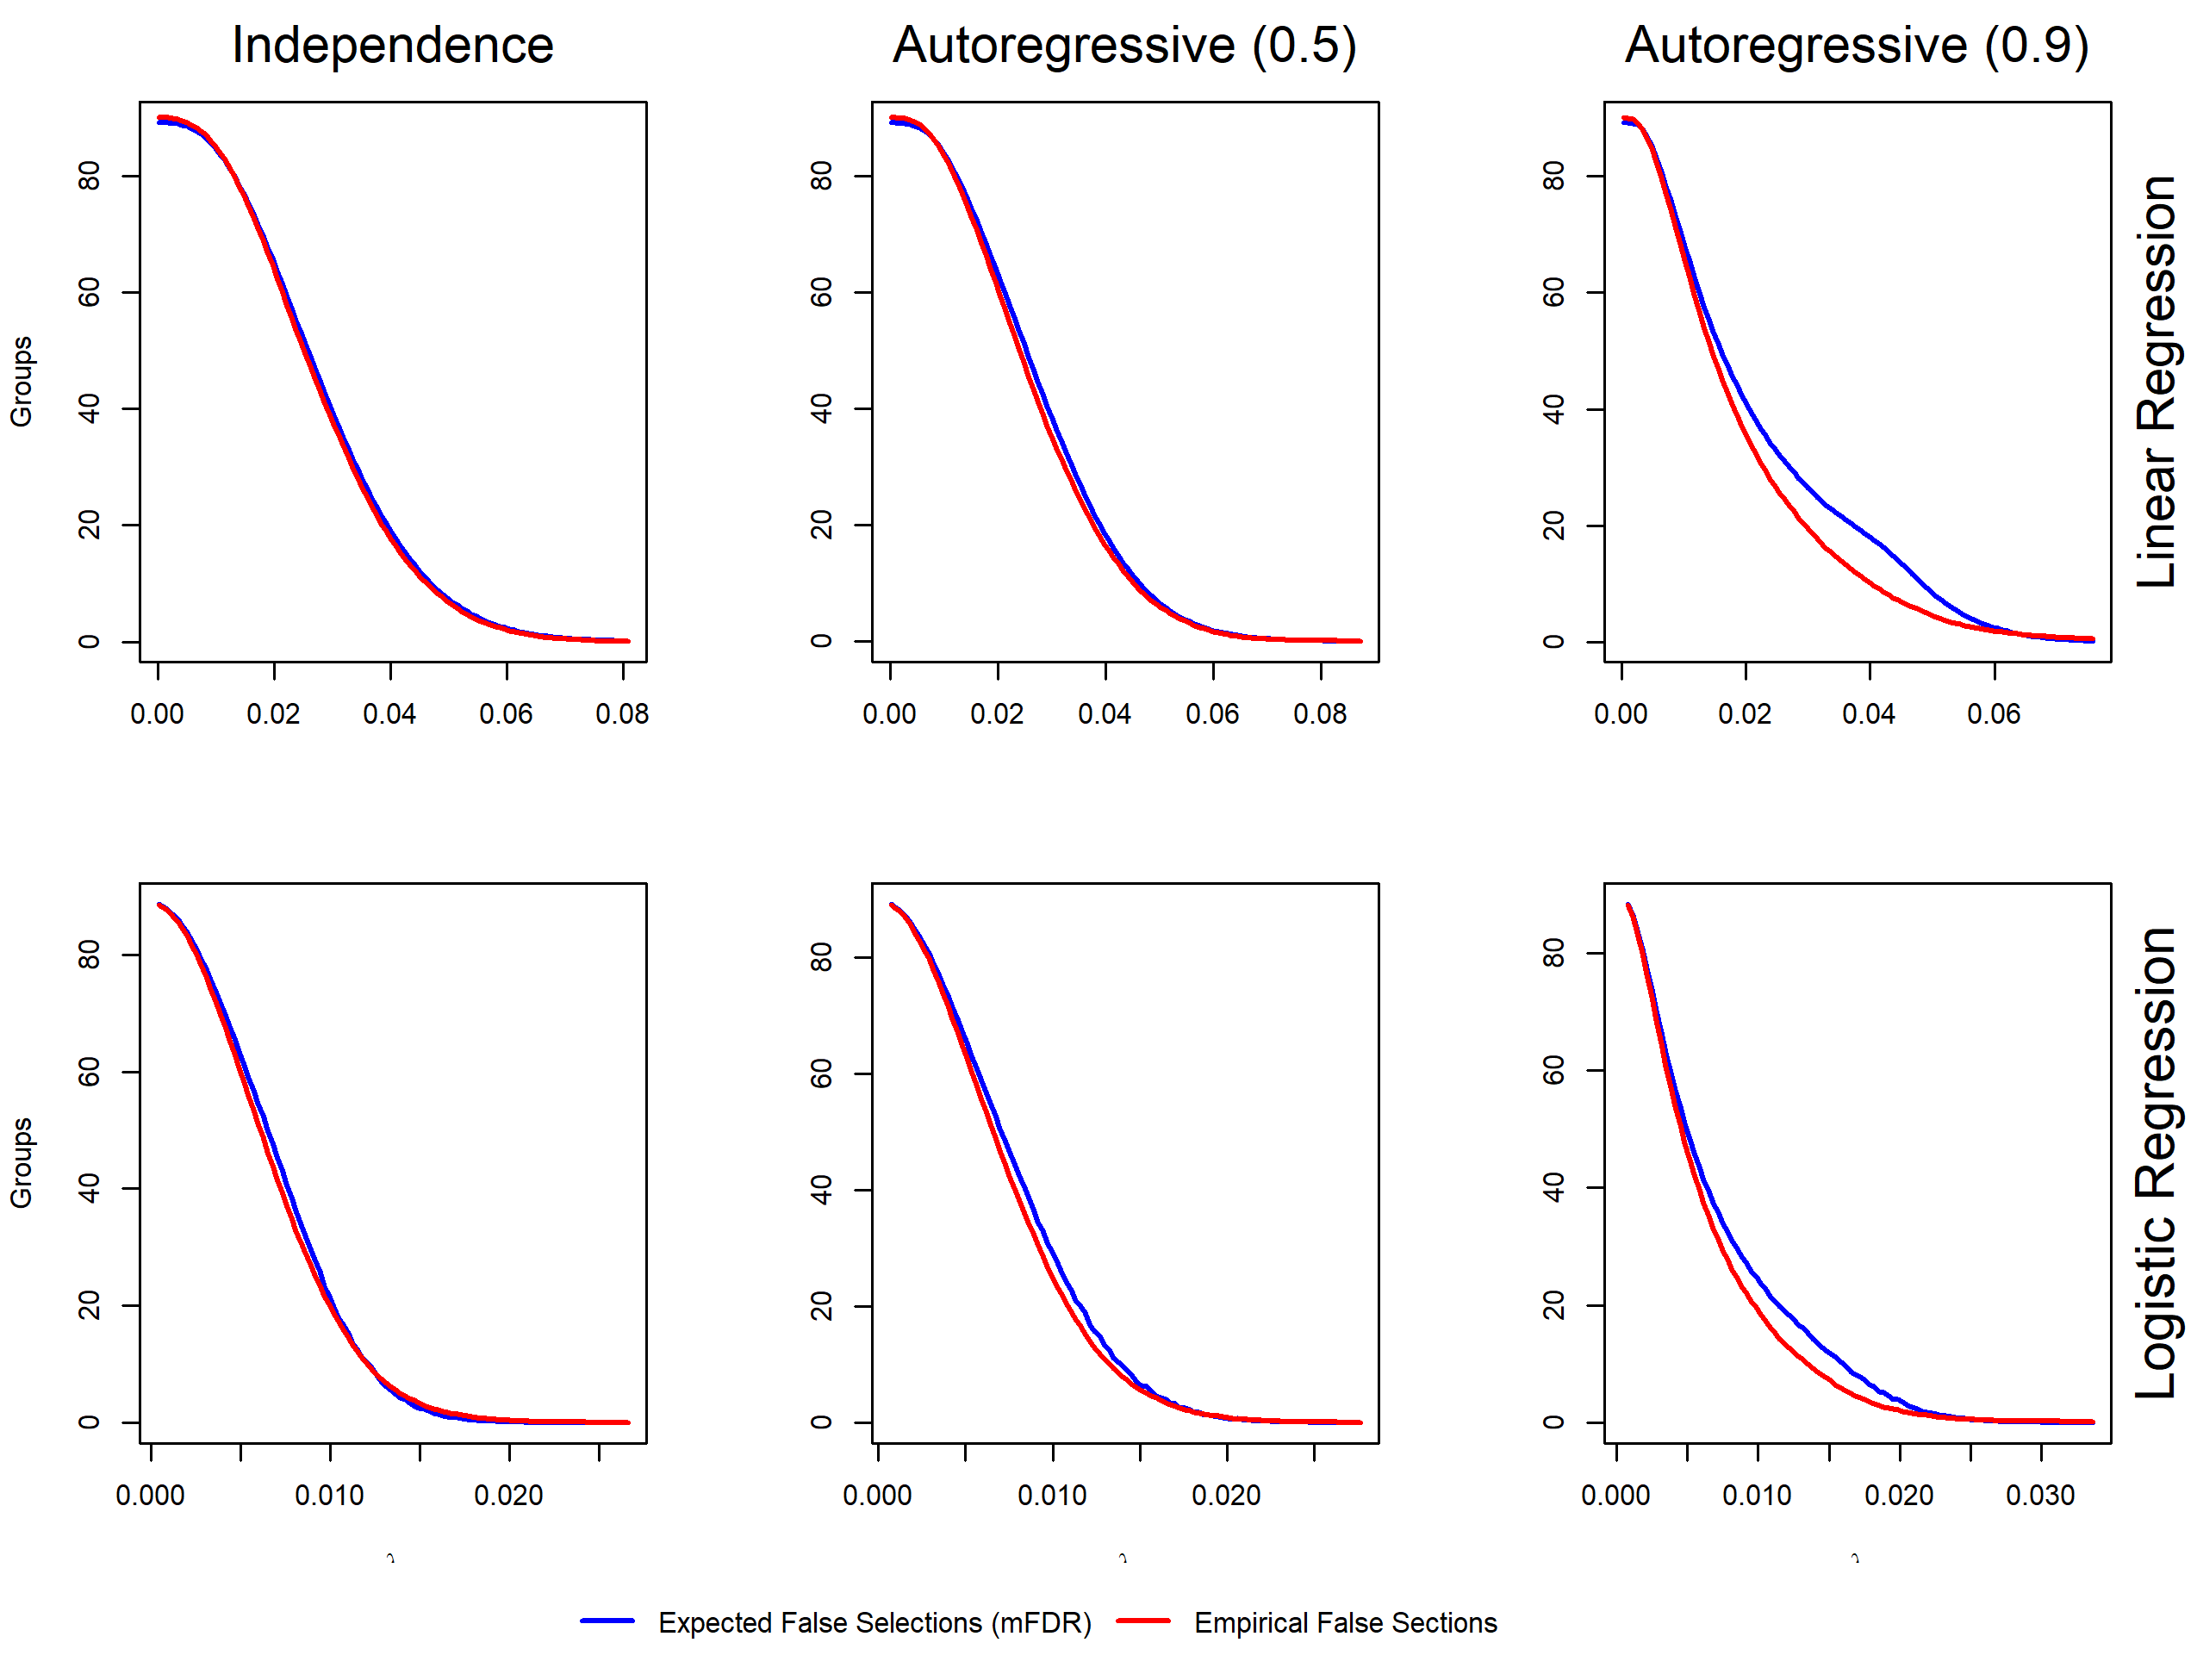
\includegraphics[width=.9\textwidth]{Fig1.png}
\caption{\label{Fig:lseq1} Comparison of the average expected and empirical number of marginal false discoveries along a sequence of $\lambda$ values for various likelihood-based models when covariates are generated independently.}
\end{figure}

Figure~\ref{Fig:lseq1} demonstrates that the expected number of false selections as estimated via Equations~\ref{eq:Mfdr} and \ref{eq:Mfdr_glm} very closely resembles the empirical number of false selections along the entire sequence of $\lambda$ values, with only a very slight degree of over-estimation induced by incidental correlations between the columns of $\X$. In the linear regression scenario, the estimated and empirical curves are nearly indistinguishable. In the logistic regression and Cox regression scenarios, the additional sources of variability discussed in Section~\ref{Sec:glm} can be observed, though the practical implications appear minimal.

\begin{figure} [!htb]
\centering
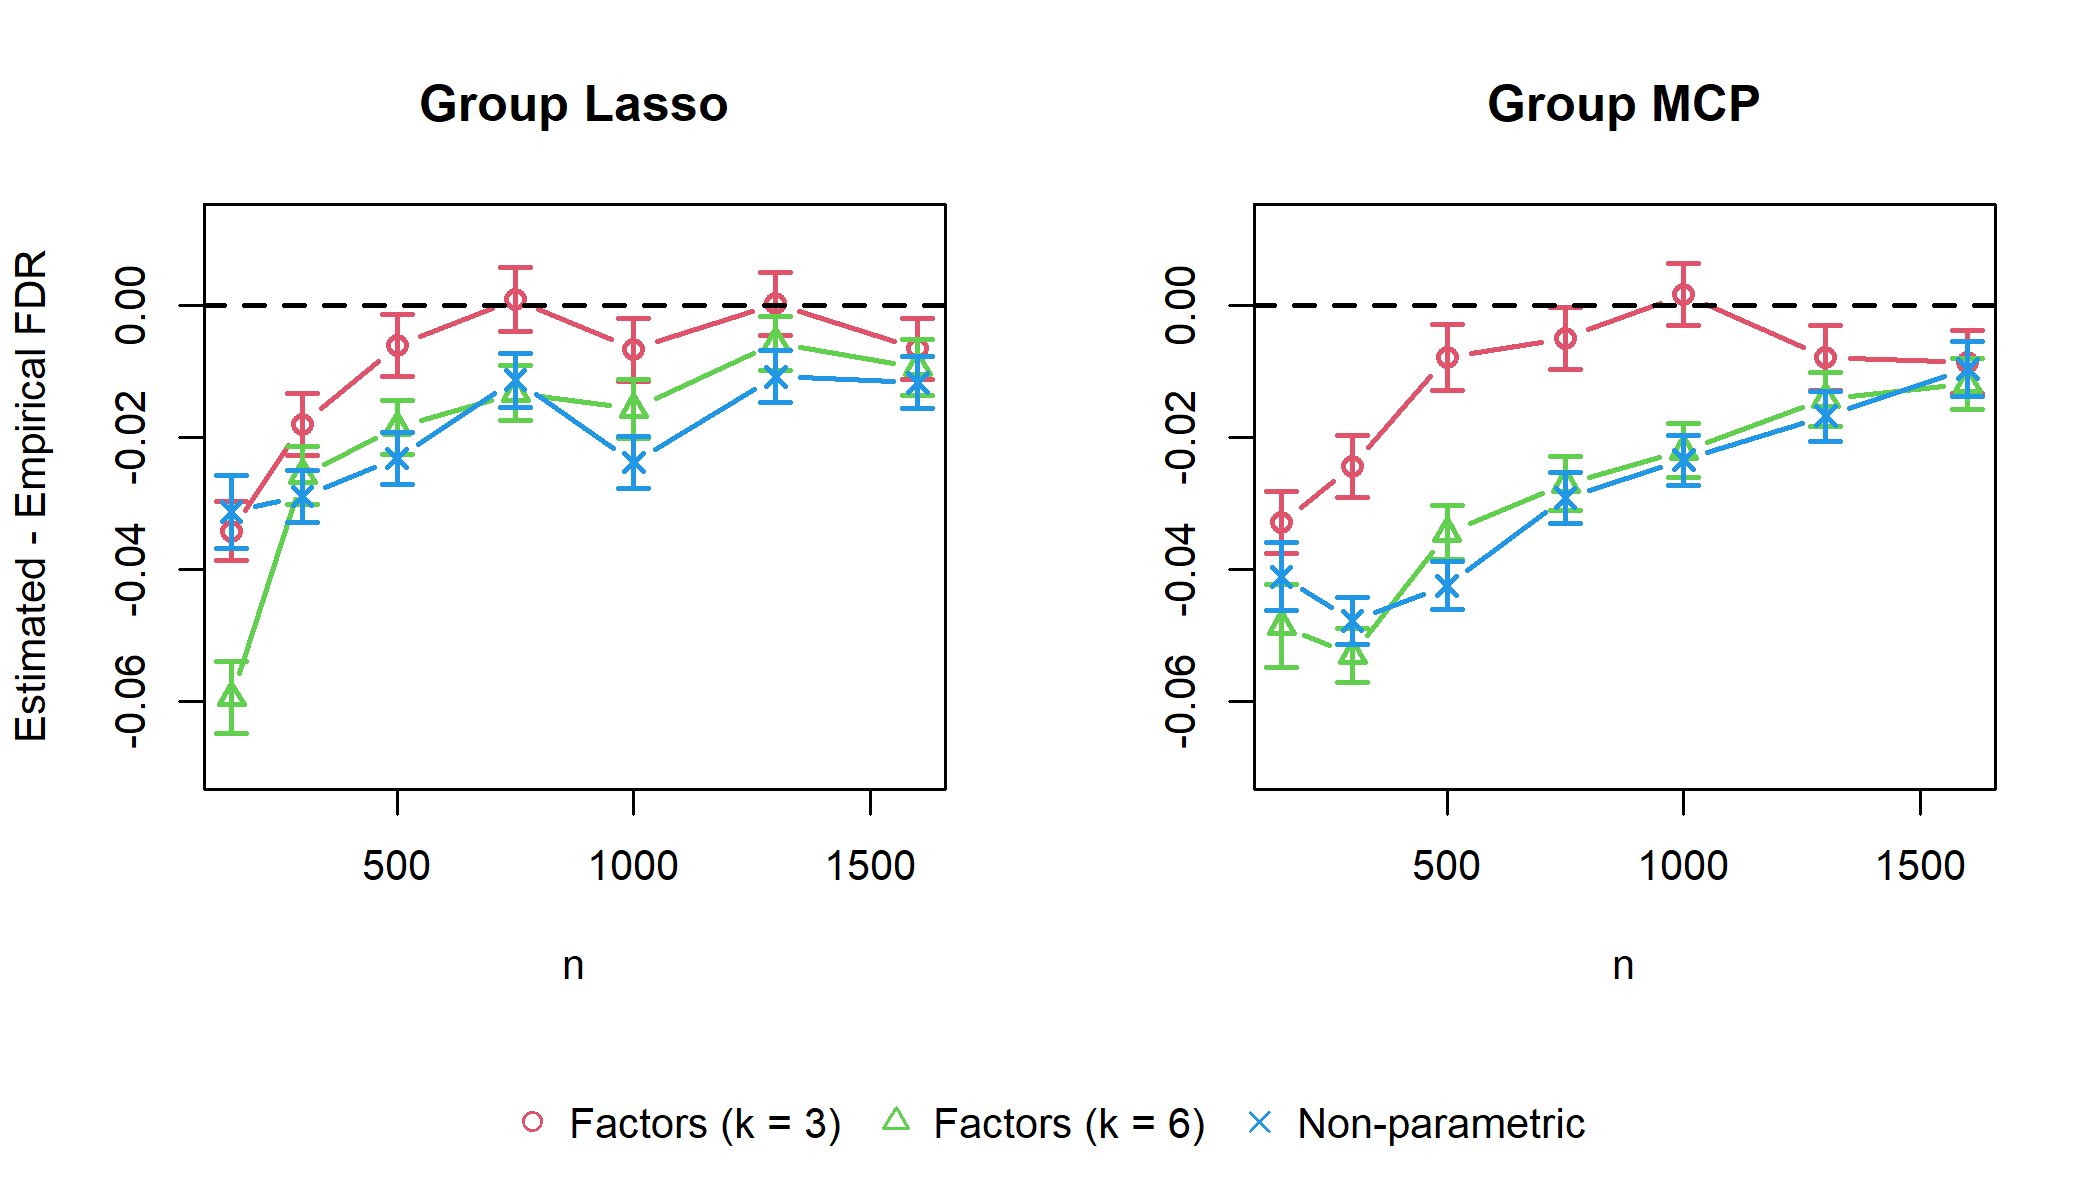
\includegraphics[width=.9\textwidth]{Fig2.png}
\caption{\label{Fig:lseq2} Comparison of the average expected and empirical number of marginal false discoveries along a sequence of $\lambda$ values for various likelihood-based models when covariates are generated using an autoregressive structure with $\rho = 0.9$.}
\end{figure}

Figure~ref{Fig:lseq2} displays the same set of curves when noise features are generated under the autoregressive correlation structure with $\rho = 0.9$.  For the reasons discussed in Section~\ref{Sec:main_meth}, the expected number of false selections estimated via Equations~\ref{eq:Mfdr} and \ref{eq:Mfdr_glm} tends to be larger than the empirical average at most values of $\lambda$, illustrating the conservative nature of these estimators in the presence of correlations between the columns of $\X$ belonging to different groups. However, in the portions of the $\lambda$ sequence that are likely of greatest interest, those where the estimated $\mFDR$ is between 10\% and 20\%, the discrepancy is relatively small in absolute terms. 

As an example, at $\lambda = 0.064$ in the linear regression setting, the average estimated marginal false discovery rate is 11.2\%, while the average empirical false discovery rate is only 8.1\%. Furthermore, even at the values of $\lambda$ that exhibit the greatest discrepancies, the estimated and empirical marginal false discovery rate tend to be close enough to lead to similar conclusions. An example of this is at $\lambda = 0.039$ in the linear regression setting, where the average estimated number of false discoveries is 19.27, which suggests the analyst should conclude that many false discoveries are to be expected among the groups selected by this model. The observed empirical average number of false discoveries at this value of $\lambda$ is 12.94, which supports the conclusion suggested by the $\mFDR$ approach.

Focusing further on the linear regression scenario under an independence correlation structure, we conduct a second set of simulation experiments that vary $n \in \{150, 300, 500, 750, 1000, 1300, 1600\}$ to evaluate the role of sample size in the accuracy of our proposed $\mFDR$ estimates.  We record the mean difference between the estimated and empirical marginal false discovery rate, averaged across 500 simulation repetitions, when selecting the smallest value of $\lambda$ with $\widehat{\text{Mfdr}} \leq 0.15$ along a fixed sequence of decreasing $\lambda$ values.  Aside from the sample size, all other aspects of this simulation are the same as those previously described in this section, with the exception that we also include results for nominal categorical predictors with groups of size $K_j = 3$ and $K_j = 6$, as well as for the group MCP penalty.

\begin{figure} [!htb]
\centering
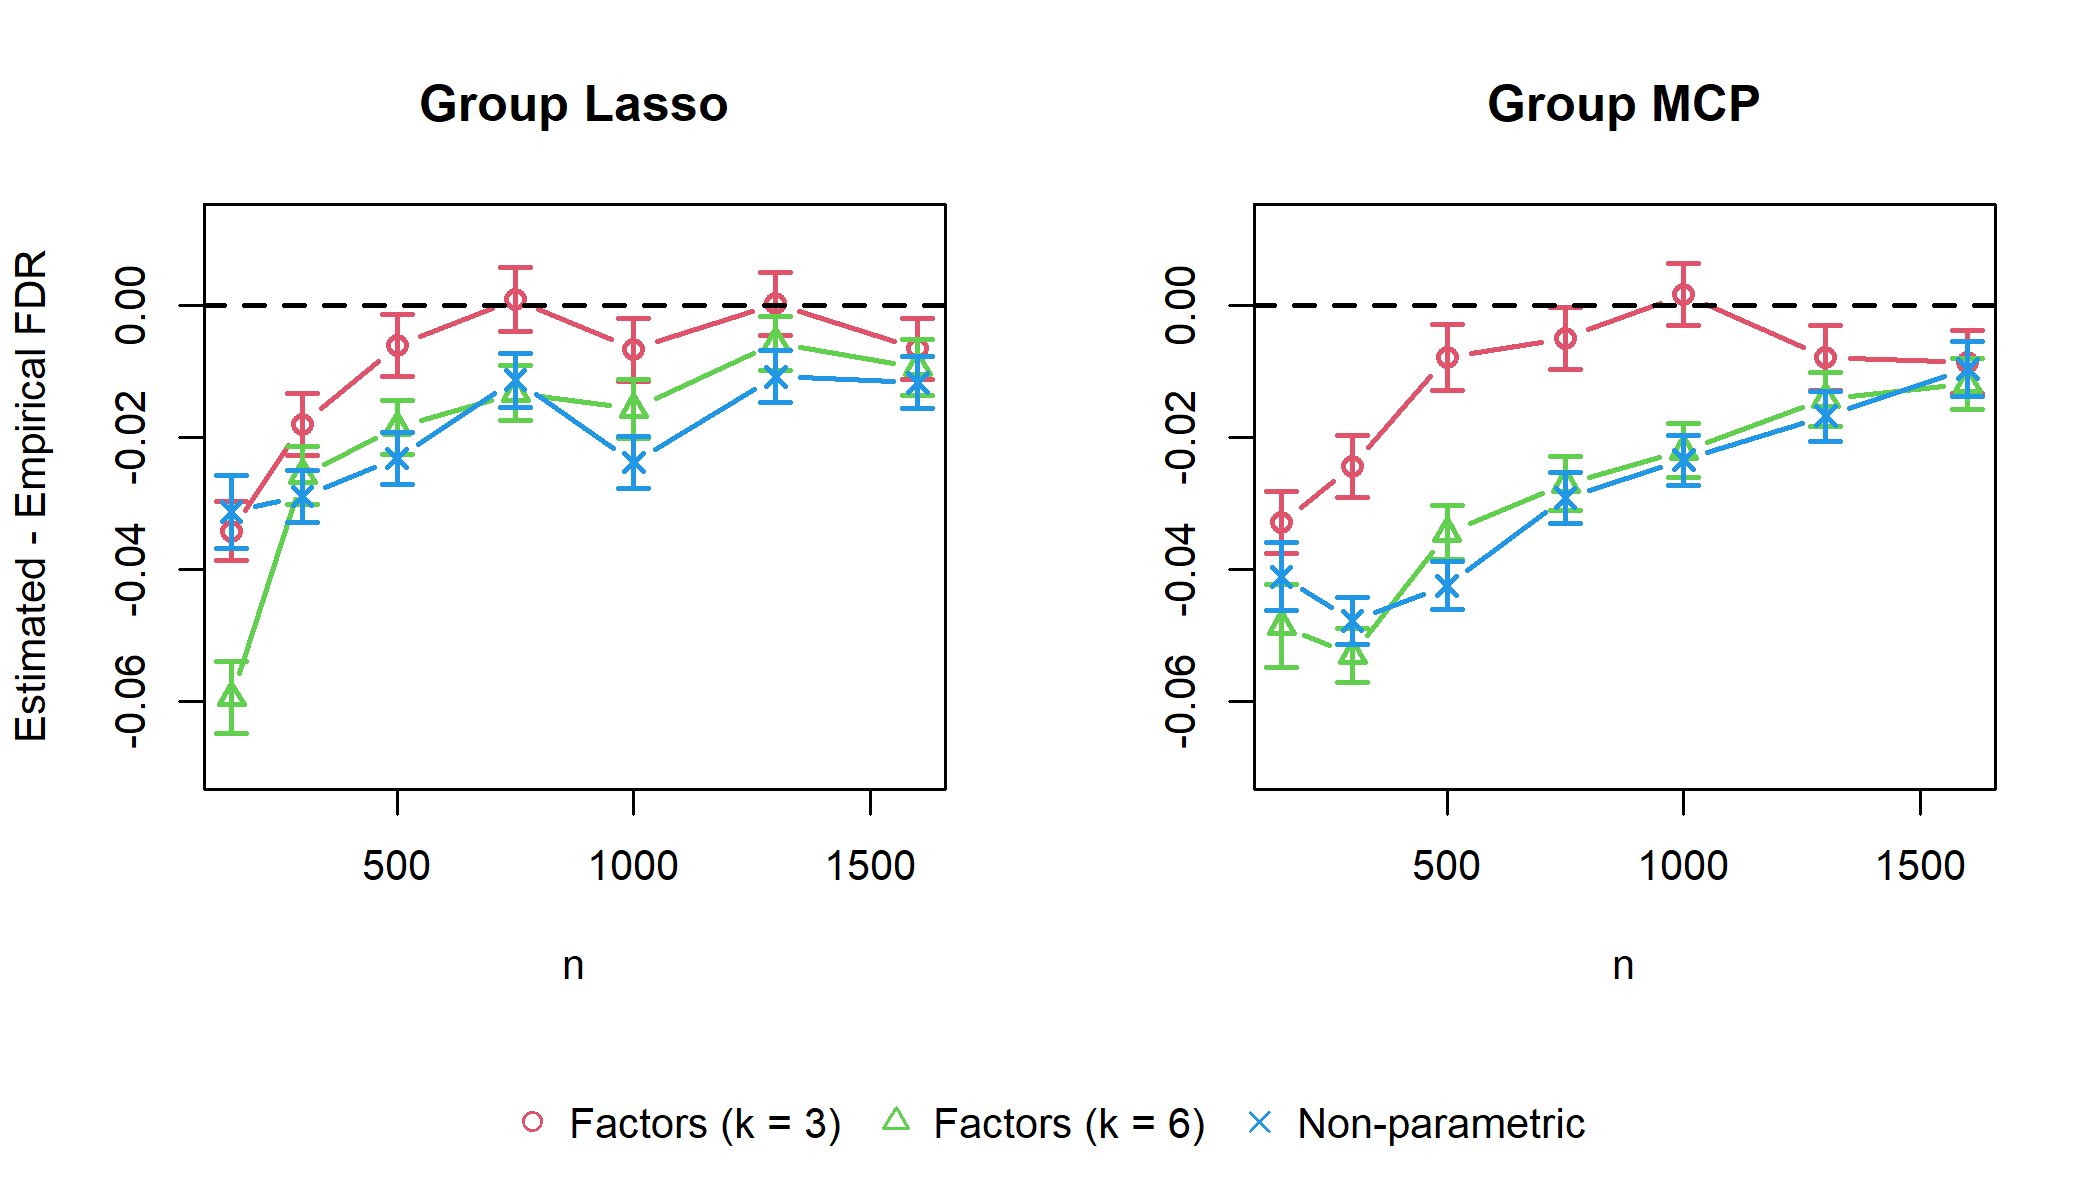
\includegraphics[width=.9\textwidth]{Fig3.png}
\caption{\label{Fig:conv} Tightness of the $\mFDR$ upper bound as $n$ increases.}
\end{figure}


Figure~\ref{Fig:conv} shows that as the sample size increases, the tightness of the $\mFDR$ bound improves.  The $\mFDR$ bound tends to be less conservative for smaller sized groups, and less conservative in applications involving categorical predictors than in non-linear additive modeling applications. In absolute terms, the degree of conservatism is small for most sample sizes, with the estimates exceeding the truth by an average of less than 0.02 in many instances.

Additionally, Figure~\ref{Fig:conv} demonstrates the applicability of our proposed $\mFDR$ method with the group MCP penalty. While the group selections and coefficient estimate under this penalization scheme tend to differ from those of the group lasso, the accuracy of our $\mFDR$ estimates tend to be comparable.  

\subsection{Comparison with other regression-based methods}
\label{Sub:comp}

Our third simulation experiment explores the ability our proposed $\mFDR$ methods to correctly identify true positives in comparison to other existing methods capable of controlling the false discover rate. We generate data using $n = 200$, consisting of $J = 100$ groups with only $t = 10$ of those groups sharing a real relationship with the outcome. We focus on the linear regression setting under the independence correlation structure, and we present the average number of true positive selections across 50 simulation repetitions for range of different signal strengths (as determined by $\beta$) while controlling the false discovery rate at 10\%. In our comparisons, consider the following methods:

\begin{itemize}[leftmargin=*, labelindent=0.5cm]
\item \textit{Forward selection with selective inference} where the selective inference approaches implemented in the {\tt groupfsInf} function contained in the {\tt selectiveInference} R package \citep{Selective_Inference} are used to obtain $p$-values for sequentially added groups.  The forward stopping rules developed by \citet{GSell2016} are then applied to these results in order to control the false discovery rate. 
\item \textit{Large-scale testing} where single group hypothesis tests are performed separately, and the results are aggregated to control the false discovery rate using the methods of \citet{BH_1995} as implemented in the {\tt p.adjust} function contained in base R.
\item \textit{Data splitting} where half of the available data is used to select groups via the group lasso with $\lambda$ chosen to minimize the 5-fold cross-validation error, and the other half is used to fit a classical least squares regression model to the selected groups and perform analysis of variance tests. The results of these tests are aggregated using the methods of \citet{BH_1995}.
\item \textit{Selective inference via the ordinary lasso} where the {\tt selectiveInference} function from the{\tt selectiveInference} R package is applied to an ordinary lasso regression model fit to the original data (before undergoing basis expansion) and the false discovery rate is controlled using forward stopping rules. This approach is only considered in the non-parametric additive modeling scenarios (those previously referred to as ``piecewise linear" and ``quadratic").
\item \textit{Knockoff filter via the ordinary lasso} where the {\tt knockoff.filter} function contained in the {\tt knockoff} R package \citep{barber2015} is applied to an ordinary lasso regression model fit to the original data (before undergoing basis expansion). This approach is also only considered in the scenarios previously referred to as ``piecewise linear" and ``quadratic".
\end{itemize}

\begin{figure} [!htb]
\centering
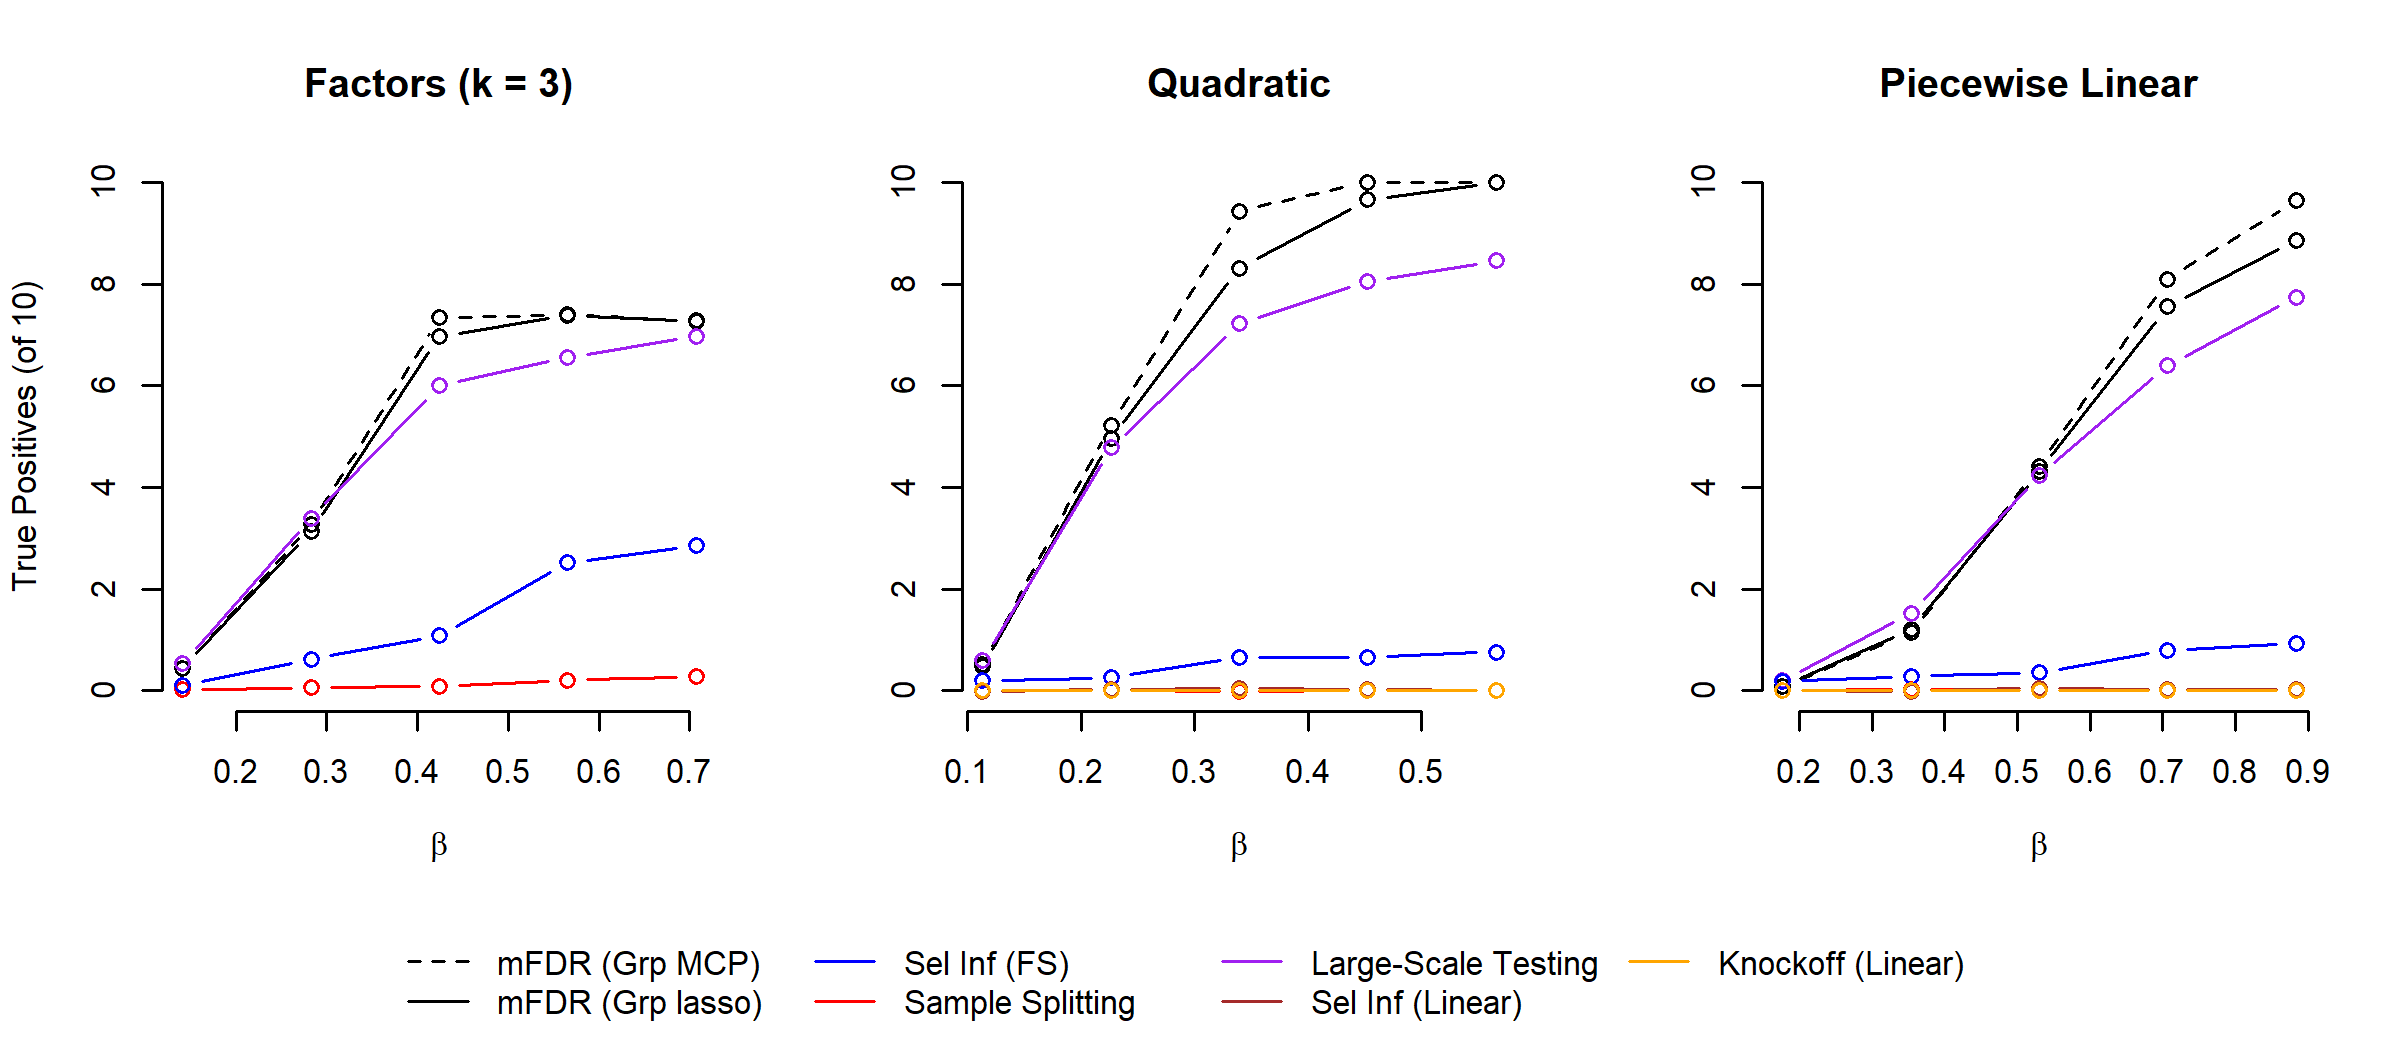
\includegraphics[width=.9\textwidth]{Fig4.png}
\caption{\label{Fig:power} The average number of true positives in response to $\beta$ for various methods of false discovery rate control applied to different linear regression applications involving $n =200$, $J = 100$, $t = 10$ and the independence correlation structure.}
\end{figure}

Figure~\ref{Fig:power} demonstrates the ability of our proposed $\mFDR$ methods to on average identify more true positives than all of the aforementioned methods. We also find that when the method is slighter more powerful when applied to models using the group MCP penalty, despite previously discussed simulations showing it to offer more conservative false discovery rate control.  Large-scale testing, which also adopts a marginal perspective on false discoveries, exhibits comparable performance when the signal size is relatively small, but falls short of $\mFDR$ for larger values of $\beta$. 

Forward selection with selective inference, which adopts a stronger pathwise perspective on false discoveries, is the only approach that on average selects at least one true positive for the values of $\beta$ we consider.  The other methods struggle to identify any of the variables that share a relationship with the outcome. These results highlight the advantages of the $\mFDR$ method and its marginal perspective on false discoveries when it comes to limiting the number of noise selections without being overly restrictive.

\subsection{Comparison with cross-validation}

Cross-validation is a resampling procedure that is commonly used to determine the optimal values of the penalty parameter(s) in penalized regression applications. Most standard penalized regression software will perform $k$-fold cross-validation, which splits the data into $k$ subsets such that model evaluation is done on data that are different from those used in model fitting. Despite its widespread use and its ability to provide an estimate of out-of-sample model performance, cross-validation will not necessarily limit the number or rate of false discoveries.

In our final simulation experiment, we compare the number of true positives and the false discovery rate of various group lasso and group MCP linear regression models for the factor ($K_j = 3$), piecewise linear, and quadratic scenarios with coefficient vectors of varying signal strength. In each scenario, we consider three different approaches for choosing $\lambda$.  The first chooses the smallest value which controls the marginal false discovery rate at 10\%, the second chooses the value that minimizes the model's 5-fold cross-validation error, and the third chooses the largest value of $\lambda$ where the cross-validation error is within 1 standard error of the minimum (referred to as the ``1se" method).  All other simulation parameters are held at the same values used in Section~\ref{Sub:comp}.

\begin{table}[htb!]
\centering
\caption{\label{Tab:cross-val} The average number of true positive selections and the average empirical false discovery rate (shown in parentheses) for various methods of choosing $\lambda$. mFDR = the smallest $\lambda$ where the estimated marginal false discovery rate is less than 10\%, CV = the value of $\lambda$ that minimizes the 5-fold cross-validation error, 1se = the largest value of $\lambda$ where the cross-validation error is within 1 standard error of the minimum. }
\vspace{.2cm}
\begin{tabular}{l l l r r r}
\hline
Penalty & Scenario & $\beta$ & mFDR & 1se & CV \\
\hline
lasso & Factors ($K_j = 3)$ & 0.2 & 1.3 (5.8\%) & 1.4 (7.4\%) & 5.2 (57.4\%) \\
& & 0.3 & 4.2 (7.5\%) & 5.5 (23.3\%) & 7.5 (65.7\%) \\
& & 0.4 & 6.3 (6.7\%) & 7.4 (30.8\%) & 8.0 (68.2\%) \\
\hline
& Piecewise Linear & 0.25 & 0.2 (4.4\%) & 0.3 (2.2\%) & 3.2 (45.9\%) \\
& & 0.5 & 3.7 (9.0\%) & 6.8 (27.9\%) & 9.2 (63.0\%) \\
& & 0.75 & 7.7 (4.8\%) & 9.8 (34.2\%) & 10.0 (67.2\%) \\
\hline
& Quadratic & 0.15 & 1.7 (4.3\%) & 2.2 (8.7\%) & 6.7 (57.3\%) \\
& & 0.2 & 3.9 (7.3\%) & 6.3 (24.8\%) & 9.2 (63.6\%) \\
& & 0.25 & 6.0 (6.7\%) & 9.1 (33.1\%) & 9.9 (66.9\%) \\
\hline
MCP & Factors ($K_j = 3)$ & 0.2 & 1.3 (6.3\%) & 0.8 (4.3\%) & 3.9 (41.3\%) \\
& & 0.3 & 4.3 (7.2\%) & 4.8 (12.5\%) & 6.7 (44.4\%) \\
& & 0.4 & \ 6.8 (7.7\%) & 7.3 (14.5\%) & 7.7 (42.9\%) \\
\hline
& Piecewise Linear & 0.25 & 0.2 (4.5\%) & 0.2 (1.4\%) & 2.0 (28.6\%) \\
& & 0.5 & 3.8 (8.9\%) & 5.2 (12.3\%) & 8.0 (35.8\%) \\
& & 0.75 & 8.4 (4.2\%) & 9.6 (12.9\%) & 9.9 (35.8\%) \\
\hline
& Quadratic & 0.15 & 1.6 (3.8\%) & 1.2 (2.5\%) & 4.6 (34.0\%) \\
& & 0.2 & 4.1 (6.4\%) & 5.1 (12.5\%) & 8.2 (39.4\%) \\
& & 0.25 & 6.4 (6.0\%) & 8.0 (14.6\%) & 9.5 (36.9\%) \\
\hline
\end{tabular}
\end{table}

The results displayed in Table~\ref{ Tab:cross-val} demonstrate the trade-off that typically occurs when choosing between a highly predictive model and a model where the analyst can be confident in importance of the selected groups.  In many scenarios, cross-validation leads to the selection of models where somewhere between 50\%-70\% of the selected groups are false discoveries.  For smaller values of $\beta$, cross-validation leads to a substantially higher number of true positives than the $\mFDR$ approach, but this diminishes as $\beta$ increases.  Additionally, the ``1se method appears to offer a middle ground; however, it does not provide any quantification of what the false discovery rate might be, and we observe real false discovery rates as high as 33\% in some scenarios when using this approach.

\section{Real data case study}

\subsection{Data}

Lung cancer is among the leading causes of death in the United States and the world, with a high mortality rate that is in part attributable to a lack of effective diagnostic tools while the disease is still in its early stages. \citet{Spira2007} studied the histologically normal bronchial epitheliums of smokers, collecting RNA expression data for $p = 22,215$ genetic features using Affymetrix HG-U133A microarrays. Among the $n = 192$ participants, 102 were cases who had already developed lung cancer and 90 were controls who had not developed lung cancer. The goal of the study was to determine whether gene expression data obtained at bronchoscopy from smokers with suspicion of lung cancer could be used as a lung cancer biomarker.

\subsection{Methods}

In our analysis we consider several different approaches using the high-dimensional genetic data to predict the binary outcome of case-control status. Our primary approach applies a basis expansion with 4 degrees of freedom to each genetic feature, creating a new design matrix, $\tilde{\X}$, that contains 88,860 columns, corresponding to 22,215 groups of size $K_j = 4$. We then use the $\mFDR$ estimator proposed in \ref{eq:Mfdr_glm} to select a group lasso model that controls the marginal false discovery rate at 10\%. 

For comparison, we conduct a large-scale univariate testing approach where separate logistic regression models are fit corresponding to each genetic feature and these models are then summarized by a likelihood-ratio test comparing their fit to that of an intercept-only model. The Benjamini-Hochberg procedure is applied to the resulting set of $p$-values to control the false discovery rate at 10\%. This approach is done separately for both the original design matrix, $\X$, and the expanded design matrix, $\tilde{\X}$. We also model the data without considering non-linear associations by fitting a lasso regression model using the binomial likelihood and applying the methods of \citet{Miller2019} to control the marginal false discovery rate. Finally, we also include results for each of the penalized regressions models favored by 5-fold cross-validation.

\subsection{Results}

\begin{table}[htb!]
\centering
\caption{\label{Tab:case-studies} A summary of various analysis approaches applied to the Spira data. S = number of selections. mFDR = estimated marginal false discovery rate (\%). MCE = cross-validated misclassification error (\%).}
\vspace{.2cm}
\begin{tabular}{l c c r r r}
\hline
Method & Design Matrix & $\lambda$ & S & mFDR & MCE \\
\hline
lasso & $\X$ & CV & 55 & 100\% & 24.5\% \\
lasso & $\X$ & mFDR & 10 & 7.8\% & 31.8\% \\
group lasso & $\tilde{\X}$ & CV & 45 & 53.4\% & 25.5\% \\
group lasso & $\tilde{\X}$ & mFDR & 21 & 5.6\% & 27.1\% \\
large-scale testing & $\tilde{\X}$ & - & 12,902 & 10.0\% & - \\
large-scale testing & $\X$ & - & 2,426 & 10.0\% & - \\
\hline
\end{tabular}
\end{table}

Table~\ref{Tab:case-studies} summarizes the results of each analysis of the Spira dataset. Among penalized regression approaches, the lowest cross-validated misclassification error is observed when the ordinary lasso used on the unexpanded design matrix; however, the estimated $\mFDR$ of this model is 100\%. Since this $\mFDR$ estimate is inherently conservative, a value of 100\% doesn't necessarily indicate that all these selections are noise; however, it does suggest that we cannot be confident in the reliability of these selections. For the ordinary lasso, controlling the marginal false discovery rate at 10\% limits the number of genetic features selected to only 10, while at the same time substantially increasing the cross-validated misclassification error. In contrast, when the group lasso is applied to the expanded design matrix, 21 genetic features can be selected while controlling the marginal false discovery rate at 10\% and achieving a misclassification error that is much closer to the minimum achieved by the ordinary lasso. 

The large-scale testing results displayed in Table~\ref{Tab:case-studies} highlight an important practical advantage of the $\mFDR$ approach. Although these methods are all based the same marginal perspective on false discoveries, the regression-based methods tend to naturally limit the number of highly correlated features that are deemed significant.  That is, in situations where many features are strongly related with both each other and the outcome, penalized regression tends to select only a single representative from the group, while large-scale testing will select all of them. In applications like this one, large-scale testing can result in an overwhelming amount of ``leads" that researchers must then filter, group, or assess manually.  In contrast, regression-based methods like $\mFDR$ tend to yield a more manageable set of features that likely contain less redundancy. 

\begin{figure} [!htb]
\centering
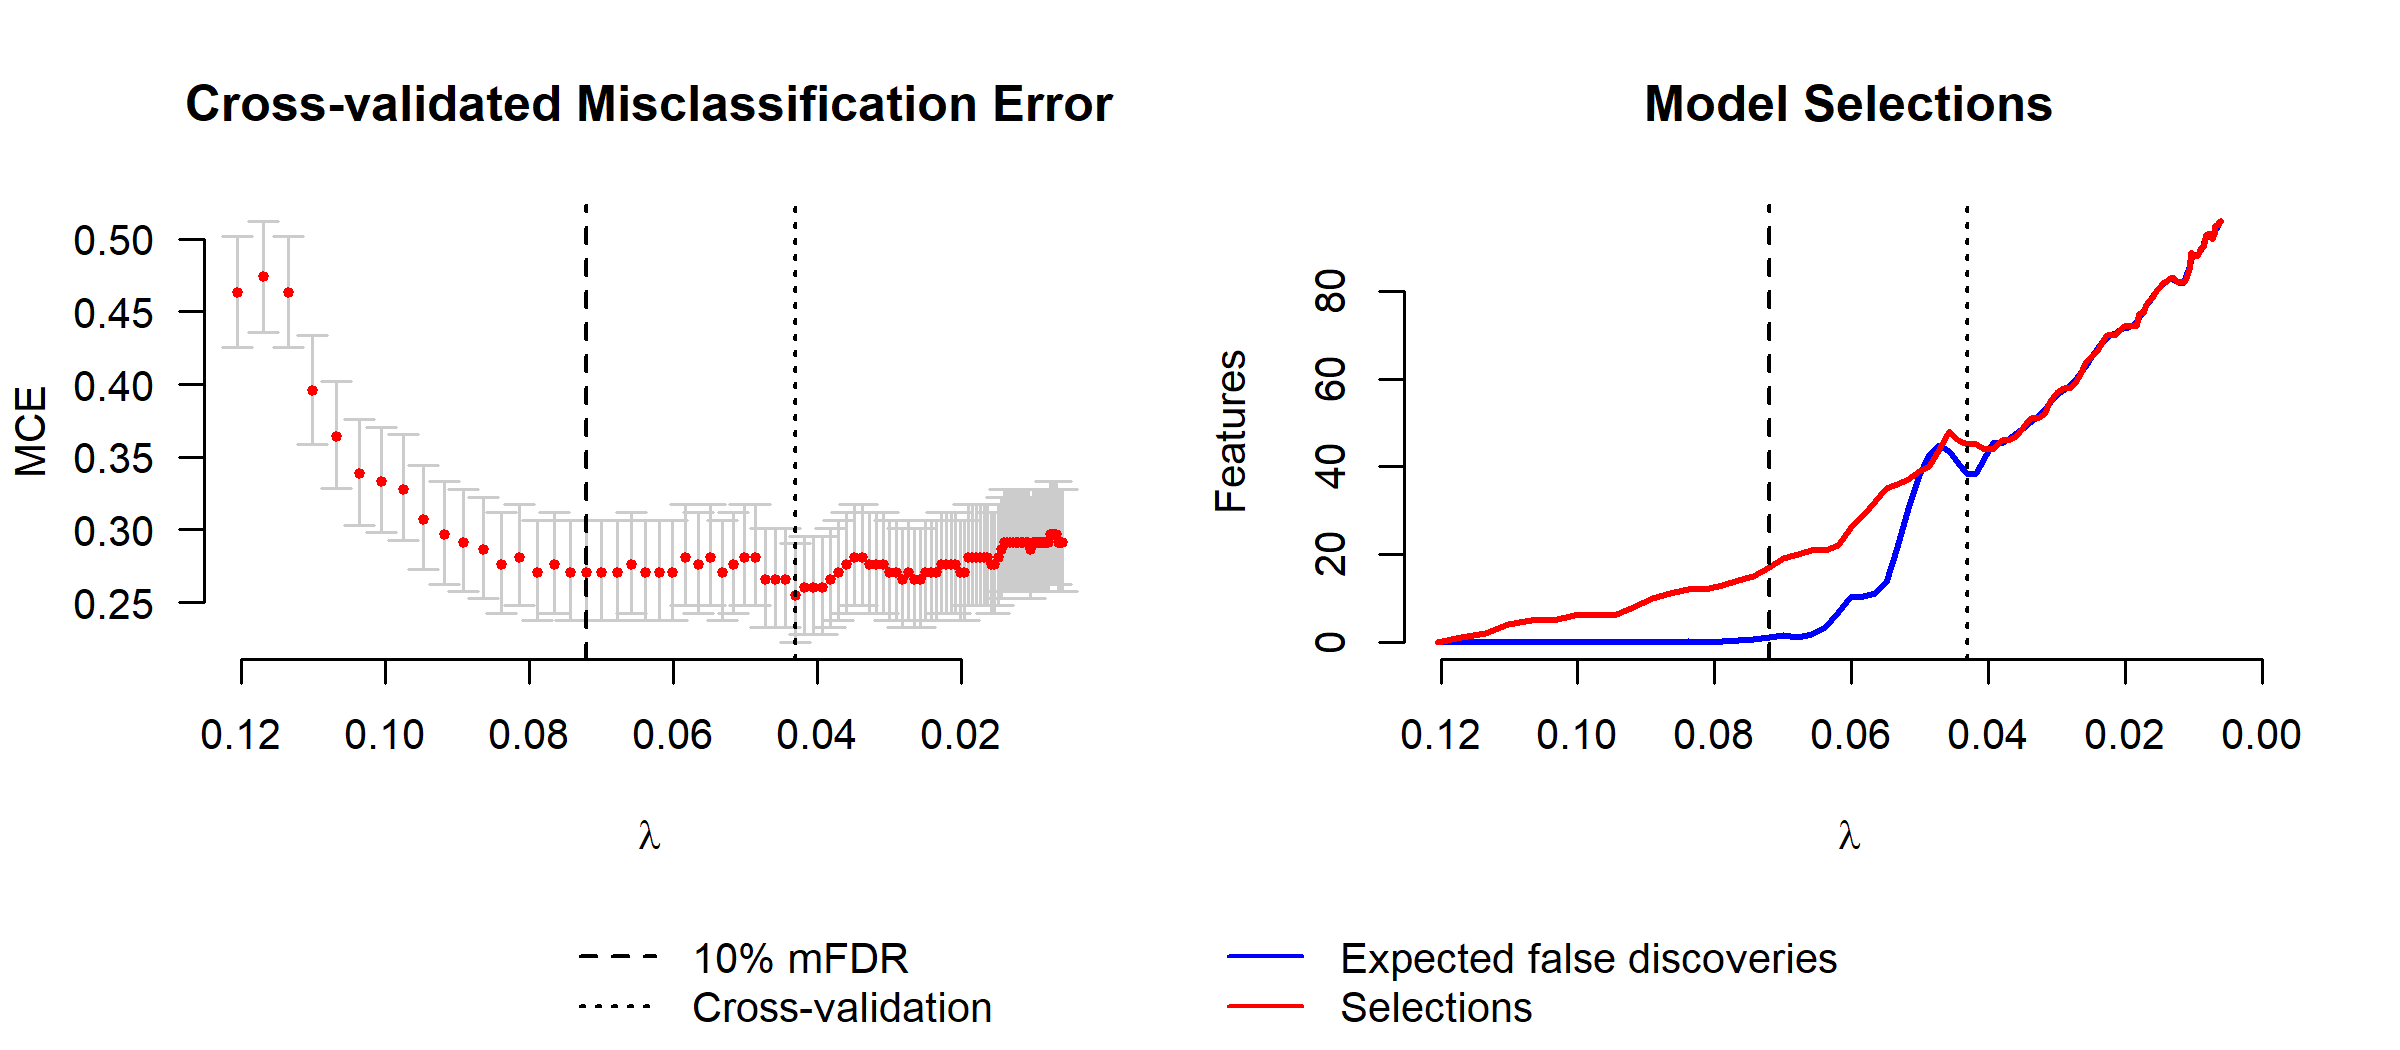
\includegraphics[width=.9\textwidth]{Fig5.png}
\caption{\label{Fig:casestudy} Group lasso modeling results for the Spira case study. The left panel displays the cross-validated misclassification error for the models corresponding to various values of a decreasing sequence of $\lambda$, while the right panel shows the total number of selections alongside the expected number of false discoveries for these models. The model favored by cross-validation marked by a dotted vertical line, while the most inclusive model with an estimated marginal false discovery rate less than 10\% marked by a dashed vertical line. }
\end{figure}

Figure~\ref{Fig:casestudy} provides a more detailed look at the results of the group lasso modeling approach. The left panel displays the cross-validated misclassification error ($\pm 1$ standard error) for models along decreasing sequence of $\lambda$ values, demonstrating a wide range of models that achieve statistically similar levels of accuracy. The right panel shows the expected number of false discoveries, calculated using the estimators in Equation~\ref{eq:Mfdr_glm}, and the total number of selections for each of these models. Together these plots can help the analyst determine a model with a suitable tradeoff between model accuracy and false discovery rate control. In this application, the improvements in misclassification error when the penalty parameter is decreased below 0.07 are relatively small and come at the cost of a substantial increase in the expected number of false discoveries present in the corresponding models.

\section{Discussion}

The ability to estimate the marginal false discovery rate of a group lasso model, or a related variant, is a useful tool in assessing the reliability of selected groups. This is particularly true when considering that many popular methods for deciding upon a group lasso model, such as cross-validation or other goodness of fit criteria, may result in undesirable numbers of false discoveries. While the $\mFDR$ approach is intended to control the marginal false discovery rate, which uses a more relaxed definition than some other methods with similar goals, it also tends to limit the number of indirect (non-causal) feature selections to much greater extent than other approaches, such as large-scale univariate testing, that adopt the same marginal perspective on false discoveries.  This makes $\mFDR$ an attractive and versatile tool in a variety of settings.

Additionally, there are very few methods of false discovery rate control that currently have readily available software implementations. The $\mFDR$ procedures described in this paper, namely those outlined in Algorithm's 1 and 2, are implemented in the {\tt grpmfdr} function that is currently available in a forked version of the `R` package {\tt grpreg} \citep{Breheny2009} which can installed directly from \url{https://github.com/remiller1450/grpreg}. Implementations are available for the linear, logistic, and Cox regression models under either the group lasso or group MCP penalty. 

From the standpoint of computational burden, the time it takes to incorporate $\mFDR$ as part of a broader analysis involving the group lasso is minimal. In the Spira case study, where the expanded design matrix contained 88,860 columns corresponding to 22,215 groups, it takes only a few minutes to estimate the number and rate of marginal false discoveries across an entire sequence of 100 $\lambda$ values.

\bigskip

\noindent {{\bf Supporting information}}

\noindent Data and source code to reproduce all results and figures are available at \url{https://github.com/remiller1450/grp_mfdr_paper}.

